%!TeX root=../pridetop.tex
\chapter[Chapter \thechapter]{}
	
\begin{figure}[t!]
\centering
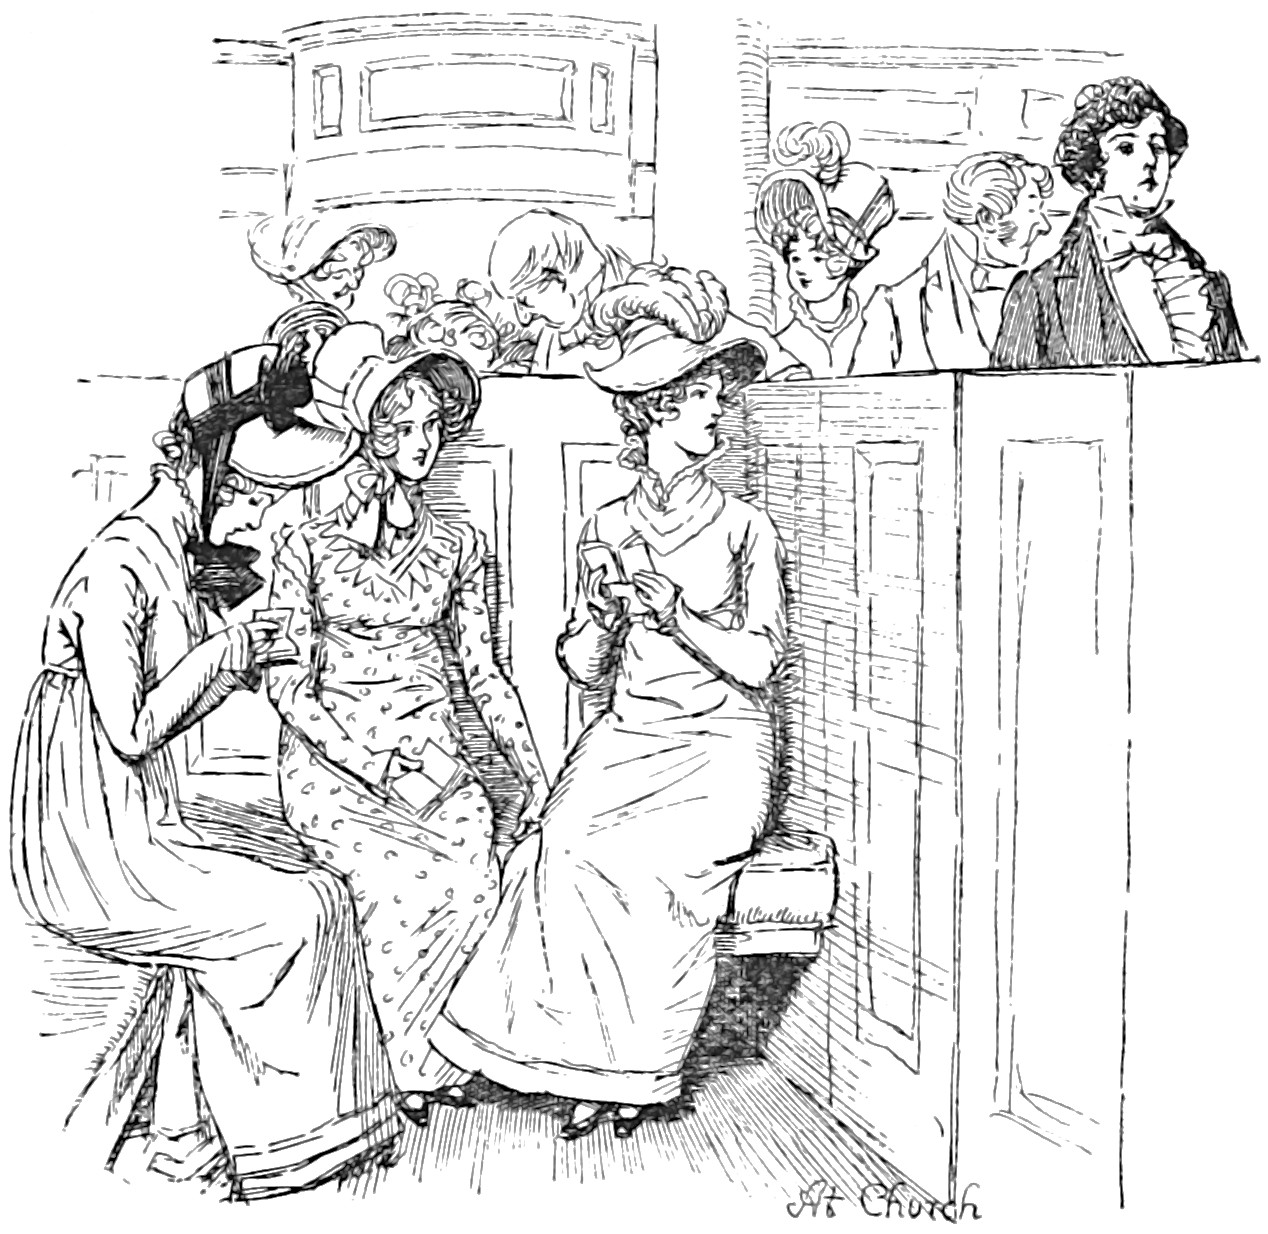
\includegraphics[width=\linewidth]{31top}
\captionlistentry{At church}
\end{figure}


\lettrine[lines=6,image=true]{initials/chap31c}{olonel}  Fitzwilliam's manners were very much admired at the Parsonage, and the ladies all felt that he must add considerably to the pleasure of their engagements at Rosings. It was some days, however, before they received any invitation thither, for while there were visitors in the house they could not be necessary; and it was not till Easter-day, almost a week after the gentlemen's arrival, that they were honoured by such an attention, and then they were merely asked on leaving church to come there in the evening. For the last week they had seen very little of either Lady Catherine or her daughter. Colonel Fitzwilliam had called at the Parsonage more than once during the time, but Mr Darcy they had only seen at church.

The invitation was accepted, of course, and at a proper hour they joined the party in Lady Catherine's drawing-room. Her Ladyship received them civilly, but it was plain that their company was by no means so acceptable as when she could get nobody else; and she was, in fact, almost engrossed by her nephews, speaking to them, especially to Darcy, much more than to any other person in the room.

Colonel Fitzwilliam seemed really glad to see them: anything was a welcome relief to him at Rosings; and Mrs Collins's pretty friend had, moreover, caught his fancy very much. He now seated himself by her, and talked so agreeably of Kent and Hertfordshire, of travelling and staying at home, of new books and music, that Elizabeth had never been half so well entertained in that room before; and they conversed with so much spirit and flow as to draw the attention of Lady Catherine herself, as well as of Mr Darcy. \textit{His} eyes had been soon and repeatedly turned towards them with a look of curiosity; and that her Ladyship, after a while, shared the feeling, was more openly acknowledged, for she did not scruple to call out,—

»What is that you are saying, Fitzwilliam? What is it you are talking of? What are you telling Miss Bennet? Let me hear what it is.«

»We were talking of music, madam,« said he, when no longer able to avoid a reply.

»Of music! Then pray speak aloud. It is of all subjects my delight. I must have my share in the conversation, if you are speaking of music. There are few people in England, I suppose, who have more true enjoyment of music than myself, or a better natural taste. If I had ever learnt, I should have been a great proficient. And so would Anne, if her health had allowed her to apply. I am confident that she would have performed delightfully. How does Georgiana get on, Darcy?«

Mr Darcy spoke with affectionate praise of his sister's proficiency.

»I am very glad to hear such a good account of her,« said Lady Catherine; »and pray tell her from me, that she cannot expect to excel, if she does not practise a great deal.«

»I assure you, madam,« he replied, »that she does not need such advice. She practises very constantly.«

»So much the better. It cannot be done too much; and when I next write to her, I shall charge her not to neglect it on any account. I often tell young ladies, that no excellence in music is to be acquired without constant practice. I have told Miss Bennet several times, that she will never play really well, unless she practises more; and though Mrs Collins has no instrument, she is very welcome, as I have often told her, to come to Rosings every day, and play on the pianoforte in Mrs Jenkinson's room. She would be in nobody's way, you know, in that part of the house.«

Mr Darcy looked a little ashamed of his aunt's ill-breeding, and made no answer.

When coffee was over, Colonel Fitzwilliam reminded Elizabeth of having promised to play to him; and she sat down directly to the instrument. He drew a chair near her. Lady Catherine listened to half a song, and then talked, as before, to her other nephew; till the latter walked away from her, and moving with his usual deliberation towards the pianoforte, stationed himself so as to command a full view of the fair performer's countenance. Elizabeth saw what he was doing, and at the first convenient pause turned to him with an arch smile, and said,—

»You mean to frighten me, Mr Darcy, by coming in all this state to hear me. But I will not be alarmed, though your sister \textit{does} play so well. There is a stubbornness about me that never can bear to be frightened at the will of others. My courage always rises with every attempt to intimidate me.«

»I shall not say that you are mistaken,« he replied, »because you could not really believe me to entertain any design of alarming you; and I have had the pleasure of your acquaintance long enough to know, that you find great enjoyment in occasionally professing opinions which, in fact, are not your own.«

Elizabeth laughed heartily at this picture of herself, and said to Colonel Fitzwilliam, »Your cousin will give you a very pretty notion of me, and teach you not to believe a word I say. I am particularly unlucky in meeting with a person so well able to expose my real character, in a part of the world where I had hoped to pass myself off with some degree of credit. Indeed, Mr Darcy, it is very ungenerous in you to mention all that you knew to my disadvantage in Hertfordshire—and, give me leave to say, very impolitic too—for it is provoking me to retaliate, and such things may come out as will shock your relations to hear.«

»I am not afraid of you,« said he, smilingly.

»Pray let me hear what you have to accuse him of,« cried Colonel Fitzwilliam. »I should like to know how he behaves among strangers.«

»You shall hear, then—but prepare for something very dreadful. The first time of my ever seeing him in Hertfordshire, you must know, was at a ball—and at this ball, what do you think he did? He danced only four dances! I am sorry to pain you, but so it was. He danced only four dances, though gentlemen were scarce; and, to my certain knowledge, more than one young lady was sitting down in want of a partner. Mr Darcy, you cannot deny the fact.«

»I had not at that time the honour of knowing any lady in the assembly beyond my own party.«

»True; and nobody can ever be introduced in a ball-room. Well, Colonel Fitzwilliam, what do I play next? My fingers wait your orders.«

»Perhaps,« said Darcy, »I should have judged better had I sought an introduction, but I am ill-qualified to recommend myself to strangers.«

»Shall we ask your cousin the reason of this?« said Elizabeth, still addressing Colonel Fitzwilliam. »Shall we ask him why a man of sense and education, and who has lived in the world, is ill-qualified to recommend himself to strangers?«

»I can answer your question,« said Fitzwilliam, »without applying to him. It is because he will not give himself the trouble.«

»I certainly have not the talent which some people possess,« said Darcy, »of conversing easily with those I have never seen before. I cannot catch their tone of conversation, or appear interested in their concerns, as I often see done.«

»My fingers,« said Elizabeth, »do not move over this instrument in the masterly manner which I see so many women's do. They have not the same force or rapidity, and do not produce the same expression. But then I have always supposed it to be my own fault—because I would not take the trouble of practising. It is not that I do not believe \textit{my} fingers as capable as any other woman's of superior execution.«

Darcy smiled and said, »You are perfectly right. You have employed your time much better. No one admitted to the privilege of hearing you can think anything wanting. We neither of us perform to strangers.«

Here they were interrupted by Lady Catherine, who called out to know what they were talking of. Elizabeth immediately began playing again. Lady Catherine approached, and, after listening for a few minutes, said to Darcy,—

»Miss Bennet would not play at all amiss if she practised more, and could have the advantage of a London master. She has a very good notion of fingering, though her taste is not equal to Anne's. Anne would have been a delightful performer, had her health allowed her to learn.«

Elizabeth looked at Darcy, to see how cordially he assented to his cousin's praise: but neither at that moment nor at any other could she discern any symptom of love; and from the whole of his behaviour to Miss de Bourgh she derived this comfort for Miss Bingley, that he might have been just as likely to marry \textit{her}, had she been his relation.

Lady Catherine continued her remarks on Elizabeth's performance, mixing with them many instructions on execution and taste. Elizabeth received them with all the forbearance of civility; and at the request of the gentlemen remained at the instrument till her Ladyship's carriage was ready to take them all home.
